\begin{comment}
							

\end{comment}

\section{Introduction}
Predicting the next item of a sequence over a finite alphabet has various approaches where some of them contain a relatively extensive literature. The applications which are covered by these various prediction approaches vary and different challenges are addressed for each one. \emph{Lossless} approach is a new approach  recently introduced by \citeauthor{gueniche_fournier-viger_tseng_2013} \citeyear{gueniche_fournier-viger_tseng_2013}. CPT credited with a fairly good ranking in SPICE (reference) competition opposite to several other \emph{lossy} approaches. However, it suffers from one major problem. Scalability is an issue that currently CPT (and its later improved version) cannot overcome. Its memory utilisations are inconsistent leading to a potentially inability to handle big amount of data. CCPT is an improved version where it successfully handles all the memory issues of CPT while offering up to 90 times less memory utilisation, memory consistency, predictability and retaining the current speed performance.
\section{Problem Definition}
Let a finite set of items (symbols) \(\Sigma = \{e_1, e_2,\ldots,e_\sigma\}\) be called \emph{alphabet}, then a \emph{sequence} \(S\) is a list of ordered items \(S=\langle i_1,i_2,\ldots,i_k\rangle\) where \(i_m \in \Sigma\ for\ 1\leq m \leq k\). A multiset of sequences \(D = \langle S_1, S_2,\ldots,S_l\rangle\) also called \emph{dataset} is constituted by sequences that created under a similar way. Given a dataset, a prediction algorithm is \emph{trained} on this dataset.  Once the prediction algorithm is trained, it will repeatedly accept a \emph{context} which is another sequence of symbols, and outputs a \emph{prediction}. The context is obtained from an unknown \emph{query sequence} which does not belong to the dataset but shares common characteristics with the dataset.  Loosely speaking, the context is derived from a part of the query sequence, and the prediction is about what comes \emph{after} the context in the query.

\section{Lossless}\label{losslessVSlossy}
Lossless sequence prediction is a relatively new approach and therefore appears to have quite a few challenges that someone that studies it has to cope with. It is clear that due to the fact that a whole dataset is utilised, a lossless approach achieves a higher space utilisation over a lossy approach. This fact leads to two results; firstly, it is somewhat intensive for an algorithm to go through all the data and extract the appropriate information needed for predictions, and secondly, keeping all the relative data \emph{in memory}, through the corresponding data structures, appears to be a considerably hard challenge because the represented structure's space utilisation often reaches an order of magnitude of the initial gathered data. As a result, a lossless sequence prediction approach needs sophisticated tools to search for patterns and sequences in \emph{Big Data} when simultaneously the aforementioned challenges are coped. CPT/CPT+ (\textbf{C}ompact \textbf{P}rediction \textbf{T}ree) introduced by \citeauthor{gueniche_fournier-viger_tseng_2013} \citeyear{gueniche_fournier-viger_tseng_2013} and later improved by \citeauthor{gueniche_fournier-viger_raman_tseng_2015} \citeyear{gueniche_fournier-viger_raman_tseng_2015}, is currently the only implementations in lossless sequence prediction. 
\par On contrary, a \emph{lossy} approach can be less memory hungry by representing the given information of a dataset through models (like \emph{dependency graphs}). This leads to implementation that sometimes utilises less space and can be potentially faster. However, a lossy approach lacks accuracy especially in hard cases when information in a dataset is not repeating as other parts of informations or a repetition is either generalised or ignored by a model having a partly loss of information that is not reversible. Often such hard cases lead to more complex models that along with Big data is hard to make algorithms that produce predictions with efficiency and performance.
\section{Motivation}
\todo{refer briefly to some SPICE results}
\\ Spice led us to the fact that CPT worths to be improved:
\\ 1.memory
\\ 2. memory consistency
\\ 3. accurate memory predictability
\\ 4. retaining fairly same speed performance
\\ 5. Able to handle efficiently more data, means EVEN better accuracy.
Current approach
\section{CPT Predictor and its Data Structures}\label{CPT}
CPT is constituted by a Trie (\emph{Prediction Tree PT}), an Array of bit-vectors (\emph{Inverted Index II}) and an array of pointers to the last items of sequences inserted to the prediction tree (\emph{Look-up Table LT}). As a lossless approach, CPT utilises the whole dataset provided for building its structures. Each sequence from the dataset is inserted to the Prediction Tree and a pointer to the last item of the sequence is added to the Look-up Table. The Inverted Index has the role of finding which sequence contains which alphabet's items by simply executing a bitwise AND operation. Every bit-vector has the same length with the total number of the dataset's sequences while it notes, using 1/0, whether an alphabet item appears in the sequence or not \ref{fig:CPT-structure}.
\par CPT can retrieve any searching sequence with specific alphabet items by using the inverted index along with a combination of the two other structures. A bitwise AND shows which sequences contain some given alphabet items and then these sequences can be located by using the Look-up Table which points to the end of each corresponding sequence. Having retrieved a requested sequence and along with the query sequence, a \emph{consequent} can be resulted as a part of the retrieved sequence. The consequent simply constitutes the sequence containing the remaining items after every item of the query (query on this case is used as a set) has been removed from the retrieved sequence. For example, if the sequence \(S_1=\langle a, b, x, z, c, d, e\rangle\) was retrieved from the prediction tree and the query sequence is \(S_q=\langle a, b, a, c\rangle\) then the consequent will be \(S_c=\langle d, e\rangle\). The produced consequent is then used by a \emph{prediction task} (see Appendix \ref{App:predtask}) in order for a prediction to get calculated.

\begin{figure}[h]
    \centering
    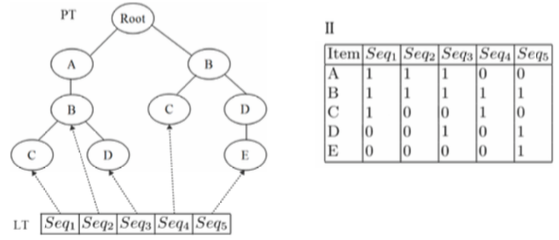
\includegraphics[width=0.75\textwidth]{CPT-structure}
    \caption{A Prediction Tree (PT), Inverted Index (II) and Lookup Table (LT)}
    \label{fig:CPT-structure}
\end{figure}

In Figure \ref{fig:CPT-structure} it is shown an example of CPT during multiple sequence insertions.

\subsection{Strengths \& Weaknesses}

CPT (as a lossless approach) utilises all the available sequences in a tree where they are accessible through the II and the LT easily and fast by a bitwise AND for each sequence. Therefore, making predictions can be potentially fast and accurate as described in \citep{gueniche_fournier-viger_tseng_2013} and \citep{gueniche_fournier-viger_raman_tseng_2015}. Locating similar sequences can be a relatively easy task that makes CPT work as a good tool for predictors that exploit such sequences. Moreover, CPT can implement all the prediction tasks described in Appendix \ref{App:predtask}, offering a bigger diversity for implementations of several applications. 
\par However, even though with the improvement of CPT, where size of the structures were reduced and speed was enhanced, some performance issues can be still addressed. Bit-vectors are the main element of II which is used for locating CPT's sequences. When more and more sequences are being added, the bitwise AND operations are becoming slower and slower, leading to performance issues and overall scalability issues since the vectors are becoming much larger. It is common for real life applications to deal with datasets that contain an enormous number of sequences. Therefore, Bit-vectors can be CPT's Achilles' heel regarding its performance (detailed performance in section \ref{experimental}). Also, space usage of II in such cases can be wasteful since with \emph{Succinct Data Structures} (see Section \ref{App:SDS}) a better and more memory efficient structure can be proposed (section \ref{ccpt}). In addition,  CPT suffers from memory consistency making it more hard to predict its behaviour in cases large datasets are utilised.
\subsection{Prediction Tree}
The prediction Tree of the CPT Predictor is constituted by a trie structure (figure \ref{fig:CPT-structure}). After the build phase where the prediction tree has been built, the main operation that the predictor needs to execute, as a part of a prediction task, is to retrieve back sequences. Which sequences will be retrieved is a matter that is decided by the II. Hence, the prediction tree is important to support instructions that give back the relative sequences. Since the LT points to the end of every sequence, it makes sense to retrieve sequences beginning from root and going up till the root. The retrieved sequence can be reversed in a later time. Therefore, a \emph{getparent()} instruction should be supported in a node of the prediction tree. Currently, the trie offers such functionality which takes \(\mathcal{O}(k)\) time for the sequence retrieval to get completed. The space required for the PT is a factor of the total number of nodes. Every node needs 32 bytes of stored information which includes a pointer to the parent node, pointers to all children nodes and the label of the node. Regardless of the space usage limitation that it is already mentioned, there is an extra limitation that can be studied in a near future. The fact that the pointers of all the children of a node are being contained in an simple array makes the build phase more and more less efficient for bigger and bigger datasets. That is because for every sequence insertion in the PT, all the children of a node has to be parsed in order to determine whether a new node insertion is required or not. A \emph{Ternary Tree} \cite{bentley_fast_1997} could solve such a problem during the building phase, but this is not yet studied.
\subsection{Inverted Index}
During prediction phase the II plays an important role in finding which sequences should be retrieved from the prediction tree. Every bit-vector of the II corresponds to an alphabet item and matches whether this alphabet item appears to a sequence or not. Every index of a bit-vector belongs to a sequence with the 0\textsuperscript{th} index to belong to the 1\textsuperscript{st} sequence of the dataset and the last index to the last sequence of the dataset. The main operation that is needed is a bit-wise AND among different bit-vectors of the II. Depending on the query sequence items, different bit-vectors are chosen from the II to apply the AND operation. The result is a bit-vector which shows which sequences contain all the query items. According to the above description, it is easy for someone to oversee that the size of the II is increasing along with the number of sequences. In a real-life application, it is usually the case that the alphabet size remains relatively stable. However, the dataset size can be increased as time passes. An example can be the fact of users' weblogs for a specific website that uses a predictor like CPT for caching web-pages. The website has a determined number of pages (constitutes the alphabet), however, the order that a user visits the pages and the amount of the pages that the user visits per session varies. Hence, different transactions are being created (constituting the sequences). Since the application lies on a lossless approach, it means that the bit-vectors of the II would take more and more space. The II is undeniably the less scalable structure to the CPT which takes \(\sigma \times l\) bits of space.
\subsection{Look-Up Table}
The Look-Up Table is the structure that adds the necessary ``glue" between the II and the Prediction Tree. After that the II will calculate which sequences contain the query items then the LT will simply point out to those sequences in the PT. The LT is an array with pointers to every end of every sequence in the PT. The pointer for the 1\textsuperscript{st} sequence is at the 0\textsuperscript{th} position of the LT, the pointer for the 2\textsuperscript{nd} sequence at the 1\textsuperscript{st} position etc. As the II, the size of the LT depends on the number of the sequences that the CPT is trained on. For every sequence, the LT uses 64 bits. In section \ref{ccpt} it will be presented a more elegant solution where the LT can be omitted completely.
\section{Succinct CPT}\label{ccpt}
Succinct CPT copes with all the memory disadvantages of CPT by introducing different succinct data structures for the roles of PT, II and LT. By using succinct data structures, fast operations like \emph{rank/select} (Appendix \ref{App:rank_select}) are offered. Thus, a significant memory reduction is achieved and performance is relatively retained.
\subsection{Elias-Fano for Inverted indicies}
The II as shown in Figure \ref{fig:CPT-structure} contains which alphabet item is contained in which sequence. However, every bit-vector can be treated as an inverted list of the positions of the set bits. Hence, the bit-vector for item \(A\) of the Figure \ref{fig:CPT-structure} can be written as \(\langle 1, 2, 3\rangle\). Since, every position in the bit-vector is correlated with a sequence serial number (1\textsuperscript{st}, 2\textsuperscript{nd}, \dots, l\textsuperscript{th} sequence) it is obvious to conclude that the aforementioned inverted list is monotone sequence of numbers. Thist is important because  the compression technique which is mainly being used and described next, is based on \emph{gap encoding}. As it will be proved later, gap encoding will make possible to store the II in space smaller or at least same as the space of the initial dataset. The techniques described below are based on a paper by Elias \cite{elias_efficient_1974} and a paper which demonstrates IIs which use such techiques \cite{vigna_quasi-succinct_2013}.
\subsubsection{Elias Techinque}
\par It is clear that every bit-vector of the II can be seen as an inverted list of the sequences that the alphabet item is contained. Because the list is monotone can be seen as \[0 \leq x\textsubscript{0} \leq x\textsubscript{1} \leq \dots \leq x\textsubscript{n - 2} \leq x\textsubscript{n - 1} \leq u \] where \(u > 0 \) as a known upper bound. That bound is always known because during prediction phase the dataset size is known too. Now, this list of numbers can be split in two bit arrays according to the formulas below:
	\begin{description}
  	\item[lower bit array:] for every item of the list, the array continuously stores its \( \lambda = max\{0, \lfloor \log(u/n)\rfloor\}\) lower bits.
  	\item[upper bit array:] then the upper bits are stored in a sequence of unary-coded gaps (see Figure \ref{fig:ef_ex})
	\end{description}

\begin{figure}[h]
    \centering
    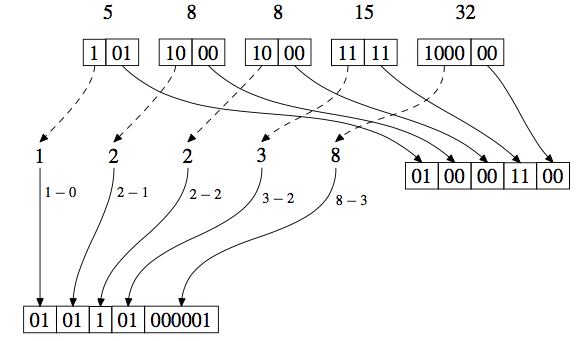
\includegraphics[width=0.75\textwidth]{elias_fano_exmpl}
    \caption{In this example we have a list of numbers 5, 8, 8, 15, 32 with upper bound 36. For the upper bit array \(\lambda = \lfloor \log36/5\rfloor = 2\). On right it is shown all the \(\lambda\) bits of all elements which are gathered together to create the lower-bets array. On left, the gaps for every number upper bits are calculated and stored sequentially in unary code in the upper-bits array.}
    \label{fig:ef_ex}
\end{figure}	
\subsubsection{Space property}
\par Space wise, it can be proven \cite{vigna_quasi-succinct_2013} that for every item of a list it is used at most \(2 + \lceil\log(u/n)\rceil\) bits. The dataset containing the sequences, from where the II will be created, can be considered as a memoryless source. Then, every symbol appears with a probability of \(p_{\kappa} = \frac{1}{\sigma} \) in the dataset. The bits needed to code a symbol will be \( \sum_{\kappa = 1}^{\sigma} p_{\kappa} \cdot \log(\frac{1}{p_{\kappa}}) = \log(\sigma)\). An II that uses Elias way of recording the set bit positions for every bit-vector, will take a total space:

\begin{equation} \label{II_ef_mem}
\sum_{\iota = 1}^{\sigma} n_{\iota}\cdot ( \log(\frac{l}{n_{\iota}}) + 2 )
\end{equation}

We set as \(M\) to be the total length of the dataset. Then:

\begin{equation} \label{II_dataset}
	M \geq l 
\end{equation} 

Using (\ref{II_ef_mem}), we can oversimplify it as:

\begin{equation}\label{II_em_simplified}
	\sum_{\iota = 1}^{\sigma} n_{\iota}\cdot ( \log(\frac{M}{n_{\iota}}) + 2 )
\end{equation}
For any bit-vector of the II:
\begin{equation} \label{bit_vector_prob}
	p_{\iota} = \frac{n_{\iota}}{M} \textnormal{, using (\ref{II_dataset})}
\end{equation}
Finally, using (\ref{II_em_simplified} and (\ref{bit_vector_prob})), the total memory of an II using Elias technique will be:

\begin{equation} \label{II_ef_mem_final}
	\sum_{\iota = 1}^{\sigma} M\cdot p_{\iota}\cdot ( \log(\frac{1}{p_{\iota}}) + 2 )
\end{equation}

In last equation (\ref{II_ef_mem_final}) and by claiming that the oversimplification at (\ref{II_em_simplified}) is usually \(M > l \), it can be assumed for most cases that the total memory is less than the memory needed to code the whole dataset. So:
\begin{equation}
	\sum_{\iota = 1}^{\sigma} M\cdot p_{\iota}\cdot ( \log(\frac{1}{p_{\iota}})) \leq M\cdot log(\sigma)
\end{equation}
This final statement is important due to the fact that most of the times a usual data structure consumes space that is a factor of the initial dataset size. In the above case, the space is usually less or the same. It is not guaranteed but experiments with real life datasets (presented in Section \ref{experimental}) follow the aforementioned behaviour is followed most of the times.
\subsubsection{Accessing Values}
\par Accessing and retrieving back any random value \(x_i\) stored with this way can be done  by following the steps on the upper bit array:
\begin{enumerate}
	\item \(\lbrack \frac{x_i}{2^{\lambda}} \rbrack = \theta \)
	\item \(\varrho = select_0(\theta)\)
	\item \(\zeta = rank_1(\varrho)\)
	\item concatenate (the binary representations) of \(\varrho - \zeta\) with the value of lower bit array at index \(\zeta\)
\end{enumerate}
Similarly, we can continue accessing all the values sequentially by keeping track of the number of the $0_s$ parsed in every position of the upper array. Every time that an $1$ is met then we have met a new stored value and therefore we should concatenate our bits. A $0$ means that we have to increase our variable that counts zeros since the gap to our next number is being increased.
\subsubsection{Instructions for CPT predictor}
CPT predictor uses the II in order to determine which sequences contain specific alphabet items. With an II which uses bit-vectors this can be done by applying a bit-wise AND to the relevant bit-vectors. In inverted indices that follow the Elias a gap encoding way, the same functionality can be achieved by \emph{decoding} every list of values for every alphabet item and them by applying an intersection among the relevant lists. However, intersecting lists that might contain a relative big amount of values is inefficient because every intersection will depend on the length of the largest list. With Elias-Fano II we can take advantage of the fact that we can \emph{jump in} a specific value of a list and complete an intersection in relation to the smallest list. Therefore, the overall speed performance is not affected much as shown in experimental evaluation.

\subsection{Prediction Tree Encoding and Storing}

\subsection{Look-Up Table Omission}
\section{Experimental Results and Performance Comparison} \label{experimental}
\subsection{Space Comparison}
\subsection{Speed Comparison}



\newpage